\chapter{Przedstawienie problemu}

\section{Drzewa decyzyjne}


%Podejmowanie decyzji jest procesem myślowym, który od początku istnienia ludzkości stwarza pewne trudności, a polega on na wybraniu najlepszego rozwiązania z dostępnych. 
Podejmowanie decyzji jest procesem nietrywialnym. Już od początku istnienia ludzkości dobrze podjęte decyzje pozwalały przeżyć wybranym grupom ludzi czy też zwierząt. Wpływ na optymalną decyzję mają informacje, które zostaną poddane analizie, ale także sama metoda analizy. Racjonalny wybór może być wspomagany różnymi algorytmami, czy też wizualną reprezentacją możliwych decyzji. Jedną z form graficznych jest drzewo decyzyjne.

Podstawowymi elementami drzewa są węzły oraz gałęzie. Korzeń drzewa to pierwszy węzeł od którego rozpoczyna się budowa całej struktury zawierającej poszczególne węzły odpowiadające za sprawdzenie pewnego warunku. Natomiast gałęzie pełnią rolę połączenia pomiędzy węzłami na kolejnych poziomach drzewa \cite{misc_1}.  Liście są końcowymi wierzchołkami drzewa i zawierają decyzje. Aby otrzymać decyzję konieczne jest przejście całego drzewa od samego korzenia do wynikowego liścia. Rezultatem takiej operacji będzie klasa decyzyjna (w przypadku drzew klasyfikacyjna) lub np. model regresyjny (w przypadku drzew regresyjnych).

\section{Uczenie maszynowe}
W otaczającym nas świecie ilość generowanych oraz gromadzonych informacji nadal przewyższa ilość danych, które można przeanalizować z użyciem obecnych zasobów. Aby analizować tak duże ilości informacji wykorzystywane są najnowsze rozwiązania technologiczne, zarówno na poziomie sprzętu komputerowego oraz oprogramowania. Dzięki zastosowaniu różnych algorytmów przetwarzania danych, klasyfikacji oraz predykcji programy komputerowe posiadają możliwość uczenia się. Tzn. uczenie maszynowe (ang. \textit{machine learning}) jest obszarem sztucznej inteligencji, który zajmuje się wykorzystywaniem komputerowego wspomagania lub podejmowania decyzji. Uczenie maszynowe w przeciągu ostatniej dekady stało się tak popularne, iż w dużej mierze zdominowało przemysł sztucznej inteligencji oraz przyczyniło się do jej rozwoju \cite{book_1}. Uczenie maszynowe stanowi trzon wielu usług, serwisów i aplikacji. Pod względem algorytmicznym odpowiada za wyniki wyszukiwania w przeglądarkach oraz za rozpoznawanie mowy przez nasze telefony. Jest także wykorzystywane w dużo trudniejszych zadaniach, jak sterowanie autonomicznymi samochodami, czy też wspomaganie lotów kosmicznych i~operacji chirurgicznych w~medycynie.

\section{Drzewa decyzyjne w technikach uczenia maszynowego}

Drzewa decyzyjne stanowią jeden z najbardziej rozpowszechnianych mechanizmów w~obszarze uczenia maszynowego. Z jednej strony mogą być wykorzystywane w zadaniach z zakresu klasyfikacji, a z drugiej strony również odgrywają ważną rolę w regresji \cite{book_1}. Mechanizm drzew decyzyjnych pozwala na budowanie modeli na podstawie ogromnych zbiorów uczących. Dodatkowym atutem drzew jest możliwość wizualnego przedstawienia sposobu dojścia do rozwiązania, które będzie zrozumiałe dla osób nie mających do czynienia z~uczeniem maszynowym i~statystyką.
% Z racji wzrostu popularności tej technologi zwiększyły się nakłady pracy naukowej w celu osiągnięcia coraz to lepszych i bardziej optymalnych algorytmów pod względem wydajnościowym. 

\subsection{System GDT}
Pracownicy Wydziału Informatyki Politechniki Białostockiej od ponad 20 lat tworzą i rozwijają narzędzie do indukowania drzew decyzyjnych, nazwane GDT (\textit{Global Decision Trees}). Narzędzie te zostało wykorzystane w pracy inżynierskiej. GDT służy do generowania drzew decyzyjnych na podstawie zbiorów wejściowych \cite{sgdt_1}. System ten jest zaimplementowany w języku C++. Podstawowa jego wersja jest programem konsolowym. Całe rozwiązanie jest unikalne, a głównym założeniem jest wykorzystanie algorytmów ewolucyjnych w procesie indukcji drzew decyzyjnych. Używając algorytmów ewolucyjnych budowane drzewa są bardziej globalne (trudniej wpaść w minimum lokalne) niż w~klasycznym podejściu. Skutkuje to możliwością osiągnięcia dokładniejszych i~lepszych wyników \cite{sgdt_2}. Algorytmy ewolucyjne wzorują się na ewolucji biologicznej \cite{book_2}. Podczas inicjalizacji parametrów algorytmu należy podać takie parametry jak wielkość populacji, prawdopodobieństwo mutacji czy też krzyżowania się danych osobników. Wartości parametrów algorytmu są określane w pliku konfiguracyjnym opartym o strukturę XML (ang. \textit{Extensible Markup Language}), który jest zarazem plikiem wejściowym do aplikacji GDT. Oprócz pliku z opcjami należy także określić pliki ze zbiorem danych:
%Pracownicy Politechniki Białostockiej również mają wkład w budowę takich rozwiązań. Autorski system GDT (\textit{Global Decision Trees}), który jest wykorzystywany w aplikacji inżynierskiej, służy do generowania modelu drzewa decyzyjnego na podstawie zbiorów wejściowych \cite{sgdt_1}. Ten system jest zaimplementowany w języku c++ oraz jest skompilowany do pliku wykonywalnego, aby umożliwić jego uruchomianie z poziomu konsoli systemu operacyjnego. Całe rozwiązanie jest unikalne, a głównym założeniem jest wykorzystanie algorytmów genetycznych. Z ich pomocą przestrzeń rozwiązań danego problemu jest większa niż w klasycznym podejściu, co skutkuje możliwością osiągnięcia dokładniejszych i lepszych wyników \cite{sgdt_2}. Metody pracy algorytmów genetycznych w dużej mierze odwzorowują działania samej natury \cite{book_2}. Podczas definiowania pracy algorytmu należy podać takie parametry jak wielkość populacji, prawdopodobieństwo mutacji czy też krzyżowania się danych osobników. Wartości tych parametrów i innych są określane w pliku konfiguracyjnym opartym o strukturę XML, który jest zarazem plikiem wejściowym do aplikacji GDT. System oprócz tego pliku wykorzystuje pliki z konkretnymi rozszerzeniami:
\begin{itemize}
	\item *.data - plik zawierający dane treningowe, 
	\item *.test - plik zawierający dane testowe,
	\item *.names - plik określających nazwy klas oraz rodzaj zmiennych.
\end{itemize}
Wykorzystując  określony zbiór trenujący oraz wartości parametrów algorytmu w pliku XML, system GDT indukuje drzewa decyzyjne. Aplikacja zapisuje do plików tekstowych statystyki wynikowe drzewa oraz użyte ustawienia parametrów.


\section{Istniejące rozwiązania}
Aktualnie na rynku można znaleźć różne aplikacje pozwalające na budowanie drzew decyzyjnych. Aplikacje te różnią się miedzy sobą zakresem funkcjonalności. Rozwiązania internetowe głównie są nastawione na zarobek, ale oferują też darmowe wersje z pewnymi ograniczeniami. Istnieją też liczne rozwiązania dla programistów w~postaci np. bibliotek dla wielu popularnych języków programowania. Takie biblioteki umożliwiają poprzez wykorzystanie modułów stworzenie podstawowych modeli uczenia maszynowego w~tym drzew decyzyjnych. Niestety ich wykorzystanie wymaga przynajmniej podstawowej wiedzy z~zakresu programowania. Dodatkowo chcąc osiągnąć bardzo wydajne rozwiązania zazwyczaj należy znać szczegóły implementacji biblioteki. Możemy także spotkać aplikacje desktopowe. Wiele takich programów jest rozwijanych przez zespoły naukowe na uniwersytetach. Do wykonania obliczeń wymagają dobrej jakości sprzętu komputerowego, który zapewni odpowiednią moc obliczeniową. 
%Aktualnie na rynku znajduje się mała liczba rozwiązań oferujących tworzenie drzew decyzyjnych. Aplikacje, które można wyróżnić różnią się między sobą zakresem funkcjonalności. Rozwiązania internetowe głównie są nastawione na zarobek, ale oferują też darmowe wersje z pewnymi ograniczeniami. Istnieją też liczne rozwiązania dla programistów w postaci paczek możliwych dla każdego z popularniejszych języków. Takie biblioteki umożliwiają w prosty sposób stworzenie podstawowych modeli uczenia maszynowego w tym drzew decyzyjnych. Negatywną cechą takiego rozwiązania jest wymagana przynajmniej podstawowa wiedza z zakresu programowania. Dodatkowo chcąc osiągnąć bardzo wydajne modele trzeba dokładnie znać mechanizmy działające pod strukturą biblioteki. Występują również nie liczne rozwiązania desktopowe. W głównej mierze są one rozwijane przez uniwersytety. Do wykonania obliczeń wymagają dobrej jakości sprzętu komputerowego, który umożliwi optymalną moc obliczeniową.    

\begin{figure}[htb]
	\centering
	
\includegraphics[width=11cm]{grafika/smartdraw.eps}
	\caption{Strona główna aplikacji \textit{SmartDraw} \cite{misc_smartdraw}.}
	\label{rys21_smartdraw}
\end{figure}

\begin{figure}[htb]
	\centering
	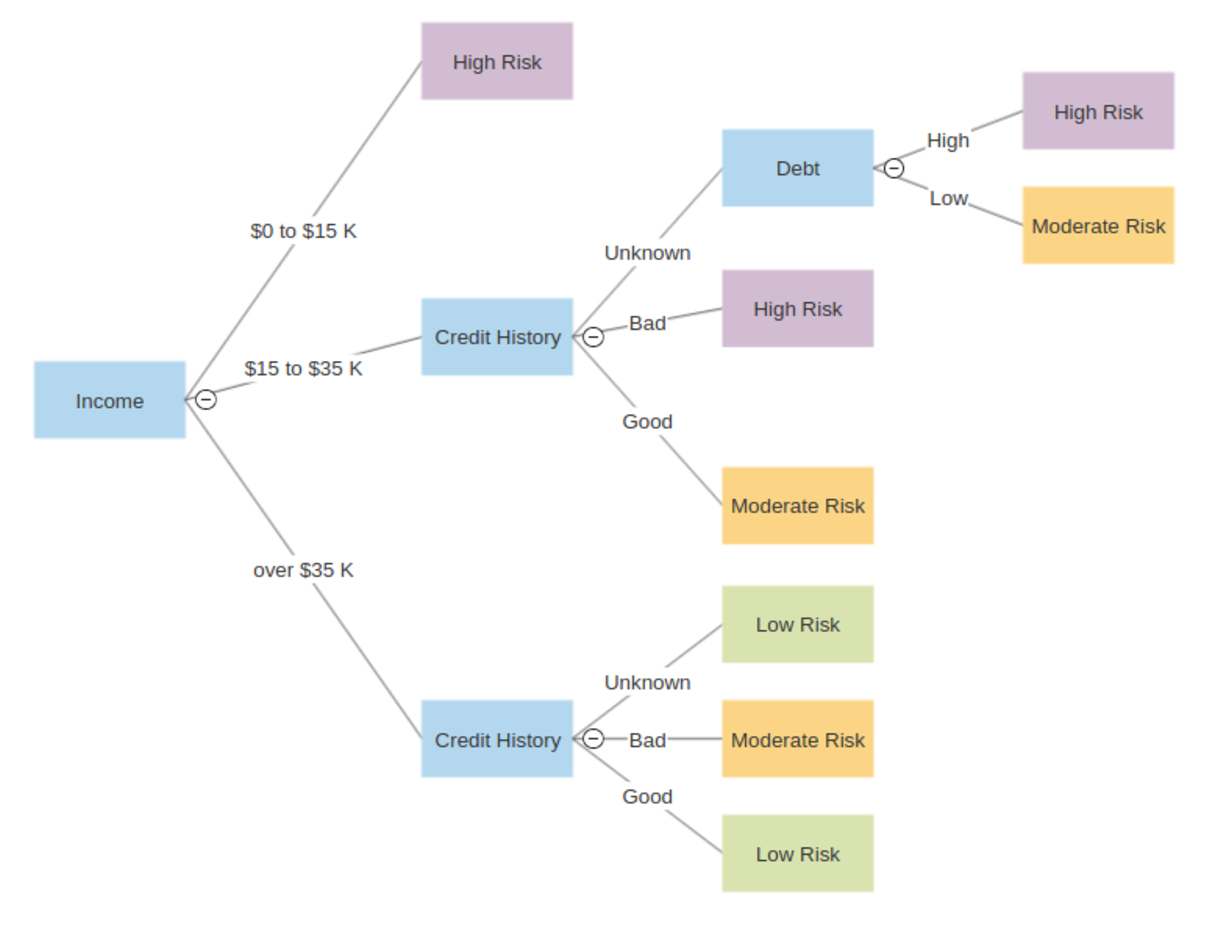
\includegraphics[width=11cm]{grafika/smartdraw_tree.eps}
	\caption{Drzewo stworzone w aplikacji \textit{SmartDraw}, źródło: opracowanie własne.}
	\label{rys22_smartdraw_tree}
\end{figure}


Aplikacja internetowa \textit{SmartDraw} jest według autora pracy jedną z wygodniejszych platform do tworzenia drzew decyzyjnych \cite{misc_smartdraw}. Użytkownik może za darmo założyć konto oraz używać aplikacji bez abonamentu przez okres próbny. Widok strony głównej został przedstawiony na Rys. \ref{rys21_smartdraw}. Platforma ponadto udostępnia funkcjonalność tworzenia innych rodzajów diagramów. Proces budowy diagramu (np. w postaci drzewa) polega na przeciąganiu i łączeniu bloków. Istnieje również możliwość wczytania struktury drzewa z~pliku o rozszerzeniu *csv (ang. \textit{comma-separated values}). Diagramy są prezentowane w~czytelny i~przejrzysty sposób (Rys. \ref{rys22_smartdraw_tree}). Ukończony diagram można wyeksportować do pliku graficznego lub dokumentu programu MS Word. Aplikacja niestety nie umożliwia budowy drzewa używając metody uczenia, jedynie pozwala na graficzne przedstawienie wcześniej przygotowanej struktury.

\begin{figure}[htb]
	\centering
	
\includegraphics[width=11cm]{grafika/canva.eps}
	\caption{Strona główna aplikacji \textit{Canva} \cite{misc_canva}.}
	\label{rys23_canva}
\end{figure}

\begin{figure}[htb]
	\centering
	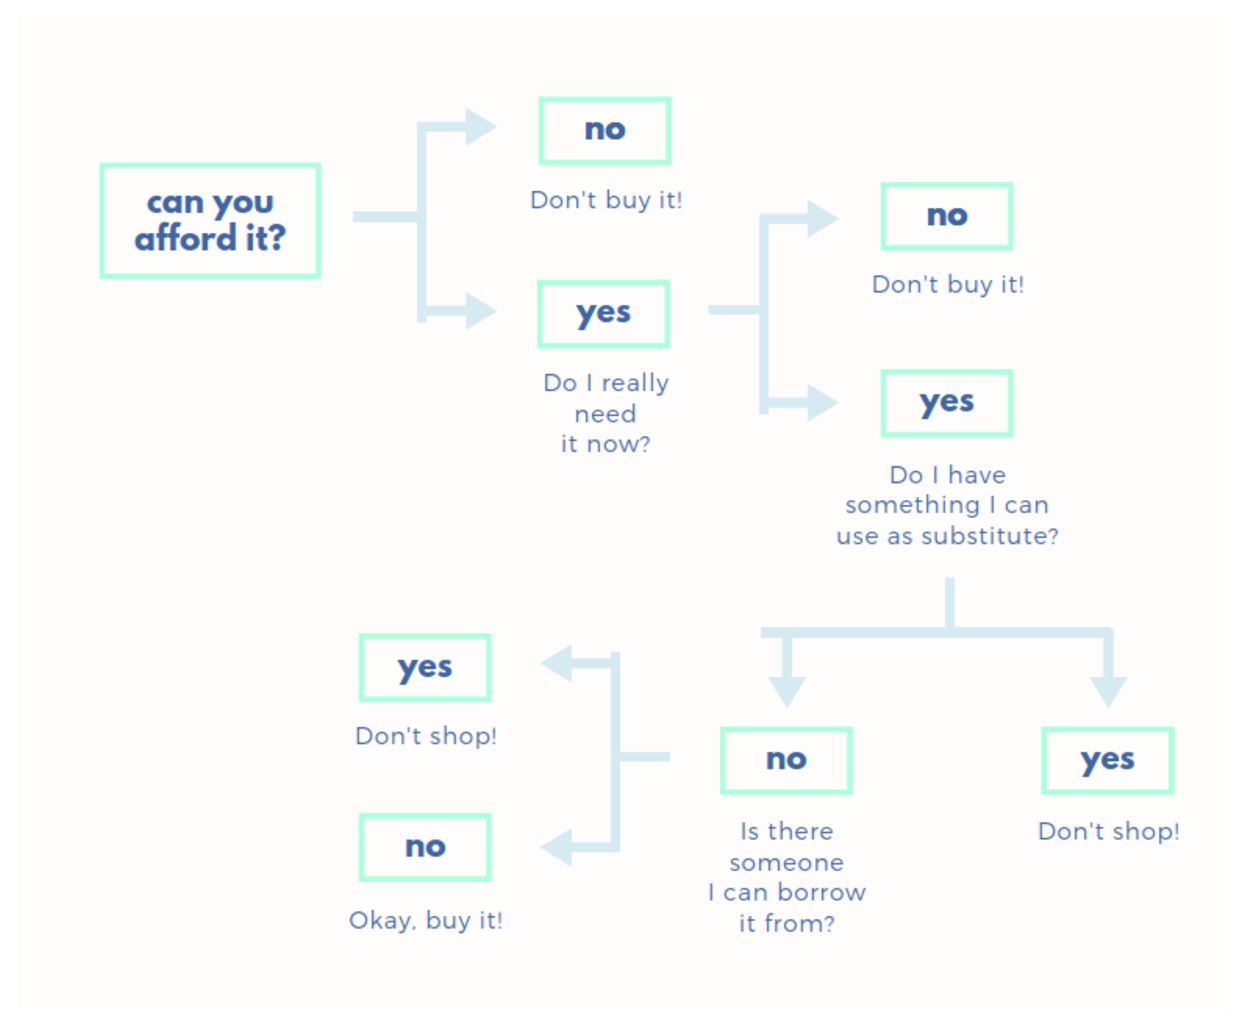
\includegraphics[width=11cm]{grafika/canvas_tree.eps}
	\caption{Drzewo stworzone w aplikacji \textit{Canva}, źródło: opracowanie własne.}
	\label{rys24_canva_tree}
\end{figure}

\textit{Canva} to kolejne narzędzie umożliwiające tworzenie drzew decyzyjnych przy pomocy przeglądarki internetowej \cite{misc_canva}. Dostęp do platformy wymaga założenia konta. Aplikacja także posiada rozszerzony, płatny pakiet funkcjonalności dla firm oraz osób prywatnych. Strona główna aplikacji została przedstawiona na Rys. \ref{rys23_canva}. Użytkownik ma możliwość wizualnego przedstawienia metodą przeciągnij i upuść (ang. \textit{drag'n drop}). W aplikacji jednak brakuje opcji indukcji drzewa decyzyjnego z wykorzystaniem zbioru uczącego. Tworzone drzewa można wzbogacić o liczne walory wizualne i dostępne gotowe motywy (Rys. \ref{rys24_canva_tree}). Głównymi odbiorcami aplikacji są reklamodawcy oraz osoby prowadzące rozbudowaną działalność w~serwisach społecznościowych. 
 
\begin{figure}[htb]
	\centering
	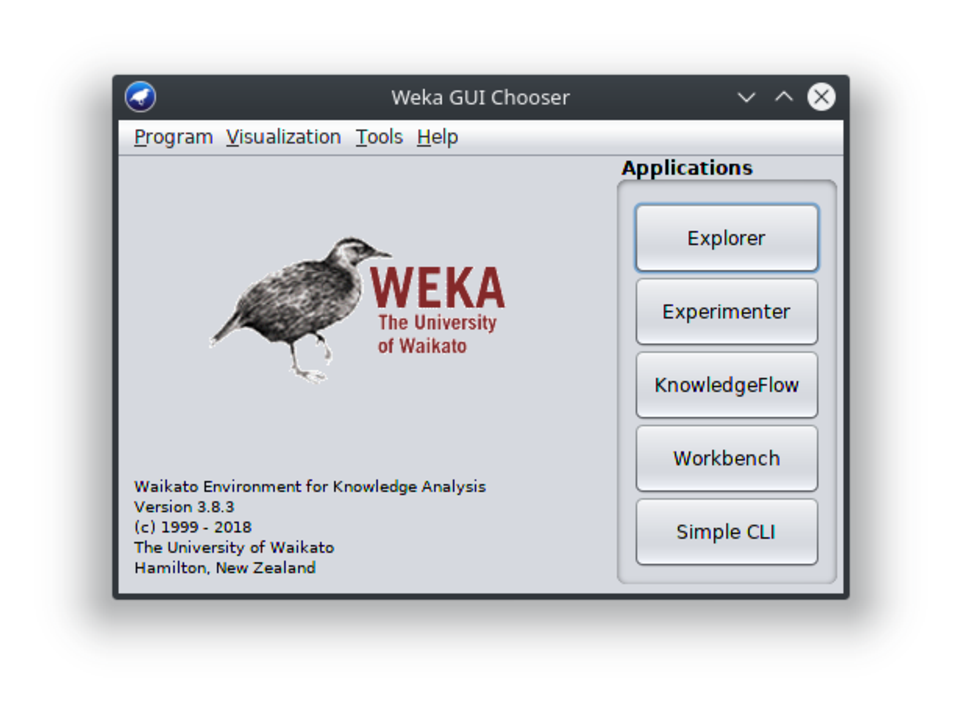
\includegraphics[height=7cm]{grafika/weka.eps}
	\caption{Okno główne aplikacji \textit{Weka}, źródło: opracowanie własne.}
	\label{rys25_weka}
\end{figure}

\begin{figure}[htb]
	\centering
	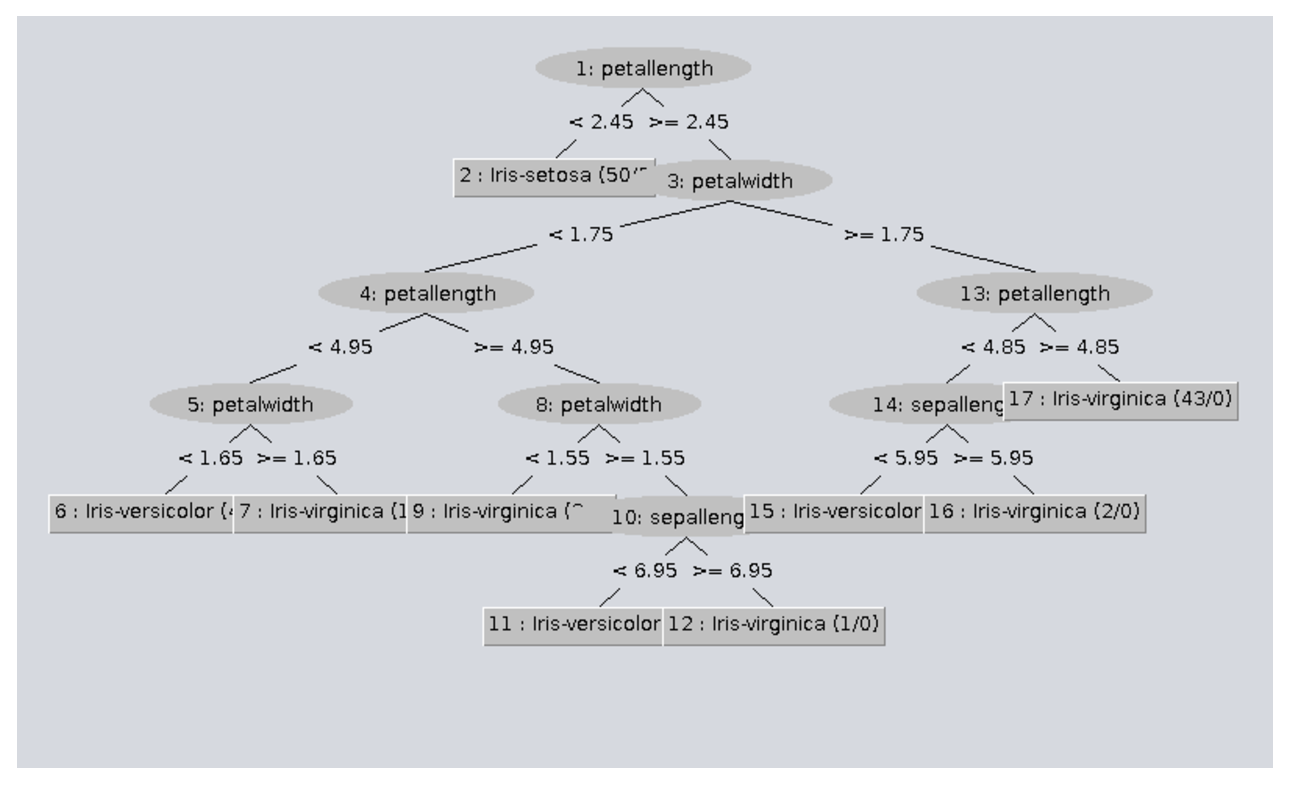
\includegraphics[width=11cm]{grafika/weka_tree.eps}
	\caption{Drzewo stworzone w aplikacji \textit{Weka}, źródło: opracowanie własne.}
	\label{rys26_weka_tree}
\end{figure}

\textit{Weka} jest aplikacją desktopową stworzoną przez naukowców zajmujących się tematami uczenia maszynowego na Uniwersytecie Waikato w Nowej Zelandii. Aplikacja została zaimplementowana w technologi JAVA SE. Pozwala to na jej uruchomienie na różnych systemach operacyjnych. Główne okno aplikacji zostało zaprezentowane na Rys. \ref{rys25_weka}. Ponadto naukowcy zaimplementowali liczne tzw. nakładki, umożliwiające korzystanie ze stworzonych mechanizmów za pośrednictwem innych języków programowania. W aplikacji użytkownik ma dostęp do dużej ilości gotowych algorytmów uczenia maszynowego, łącznie z algorytmami indukcji drzew decyzyjnych. Tworzenie nowego eksperymentu zaczyna się od wybrania zestawu danych. Użytkownik początkujący może skorzystać z przykładowych plików. Po wczytaniu zbioru wejściowego istnieje możliwość wizualizacji danych oraz ich wstępnej obróbki. W kolejnym kroku użytkownik wybiera algorytm budowy klasyfikatora. Do wyboru jest kilka różnych algorytmów związanych z tworzeniem drzew decyzyjnych. Czas obliczeń zależy od ilości danych, wybranego algorytmy oraz posiadanych zasobów obliczeniowych. Rezultaty eksperymentu są przedstawiane w postaci tekstowej. Istnieje także możliwość wyświetlenia drzewa graficznie. Przykładowe drzewo decyzyjne stworzone za pośrednictwem programu zostało przedstawione na Rys. \ref{rys26_weka_tree}.

Aplikacja tworzona w ramach pracy dyplomowej jest aplikacją oryginalną. Po pierwsze ze względu na wykorzystany system GDT. Po drugie, będzie to aplikacja internetowa, która umożliwi indukowanie drzew decyzyjnych z wykorzystaniem algorytmów ewolucyjnych. To co będzie ją odróżniać to moduł do zarządzania zadaniami, które będą uruchamiać się zdalnie, przez co użytkownik końcowy nie będzie musiał posiadać znaczących zasobów pamięciowych i~obliczeniowych. Budowane narzędzie pozwoli także na graficzną i~interaktywną reprezentacje otrzymanych wyników.
% Ponadto poszczególne atrybuty węzłów zostają zobrazowane za pośrednictwem wykresów. Aplikacja umożliwia również liczne modyfikacje w parametrach algorytmów mające na celu osiągniecie lepszych wyników.  
%Rozwiązanie oferowane przez pracę dyplomową jest unikalne nie tylko ze względu na wykorzystany system GDT. Wyróżnia się w pełni niezależnością użytkownika od sprzętu, który posiada, co w przypadku takich rozwiązań jak program \textit{Weka} ma znaczenie. Aktualnie dostępne rozwiązania internetowe nie wyróżniają się miedzy sobą sposobem działania,a dodatkowo umożliwiają ograniczone funkcjonalności co do budowania drzew na podstawie zbiorów danych. Natomiast rozwiązania desktopowe wymagają od użytkownika dużej znajomości tego zagadnienia. Aplikacja powstała podczas pracy dyplomowej wypełnia lukę na rynku. Umożliwia darmowy, łatwy pod względem obsługi system dla użytkownika, nawet który dopiero zaczyna przygodę z uczeniem maszynowym. Co więcej rozszerza o takie funkcjonalności jak udostępnianie eksperymentów i przejrzysty sposób zarządzania nimi. 